% !TeX program = lualatex
\documentclass[11pt]{article}

\usepackage[a4paper,margin=0mm]{geometry}
\usepackage{fontspec}
\usepackage{graphicx}
\usepackage{tikz}
\usepackage{xcolor}
\usepackage[colorlinks=true,urlcolor=blue]{hyperref}

\setmainfont{DejaVu Sans}
\definecolor{openroadgreen}{HTML}{3F8A49}
\pagestyle{empty}
\setlength{\parindent}{0pt}

\newcommand{\checkitem}[2]{
  \node[anchor=west,text=openroadgreen,font=\bfseries\fontsize{16}{16}\selectfont] at (14mm,-#1) {✔};
  \node[anchor=west,text=black,font=\bfseries\fontsize{11.5}{13.5}\selectfont] at (22mm,-#1) {#2};
}

\begin{document}
\begin{tikzpicture}[remember picture,overlay]
\begin{scope}[shift={(current page.north west)}]

  \node[anchor=north west,text=black,font=\bfseries\fontsize{29}{32}\selectfont] at (14mm,-13mm) {HOTPOT:};
  \node[anchor=north west,text=black,font=\fontsize{20}{23}\selectfont] at (14mm,-30mm) {A \textbf{H}ands-\textbf{O}n \textbf{T}utorial for \textbf{P}hysical};
  \node[anchor=north west,text=black,font=\fontsize{20}{23}\selectfont] at (14mm,-43mm) {Design with \textbf{O}pen-Source \textbf{T}ools};

  \node[anchor=north east,inner sep=0] at (196mm,-13mm) {
\includegraphics[width=39mm]{poster-assets/uni-bonn-logo.pdf}};

  \node[anchor=north,text=black,font=\bfseries\fontsize{15}{17}\selectfont] at (105mm,-58mm) {21-23 September 2026 \quad Monday-Wednesday};

  \node[anchor=center,inner sep=0] at (105mm,-130mm) {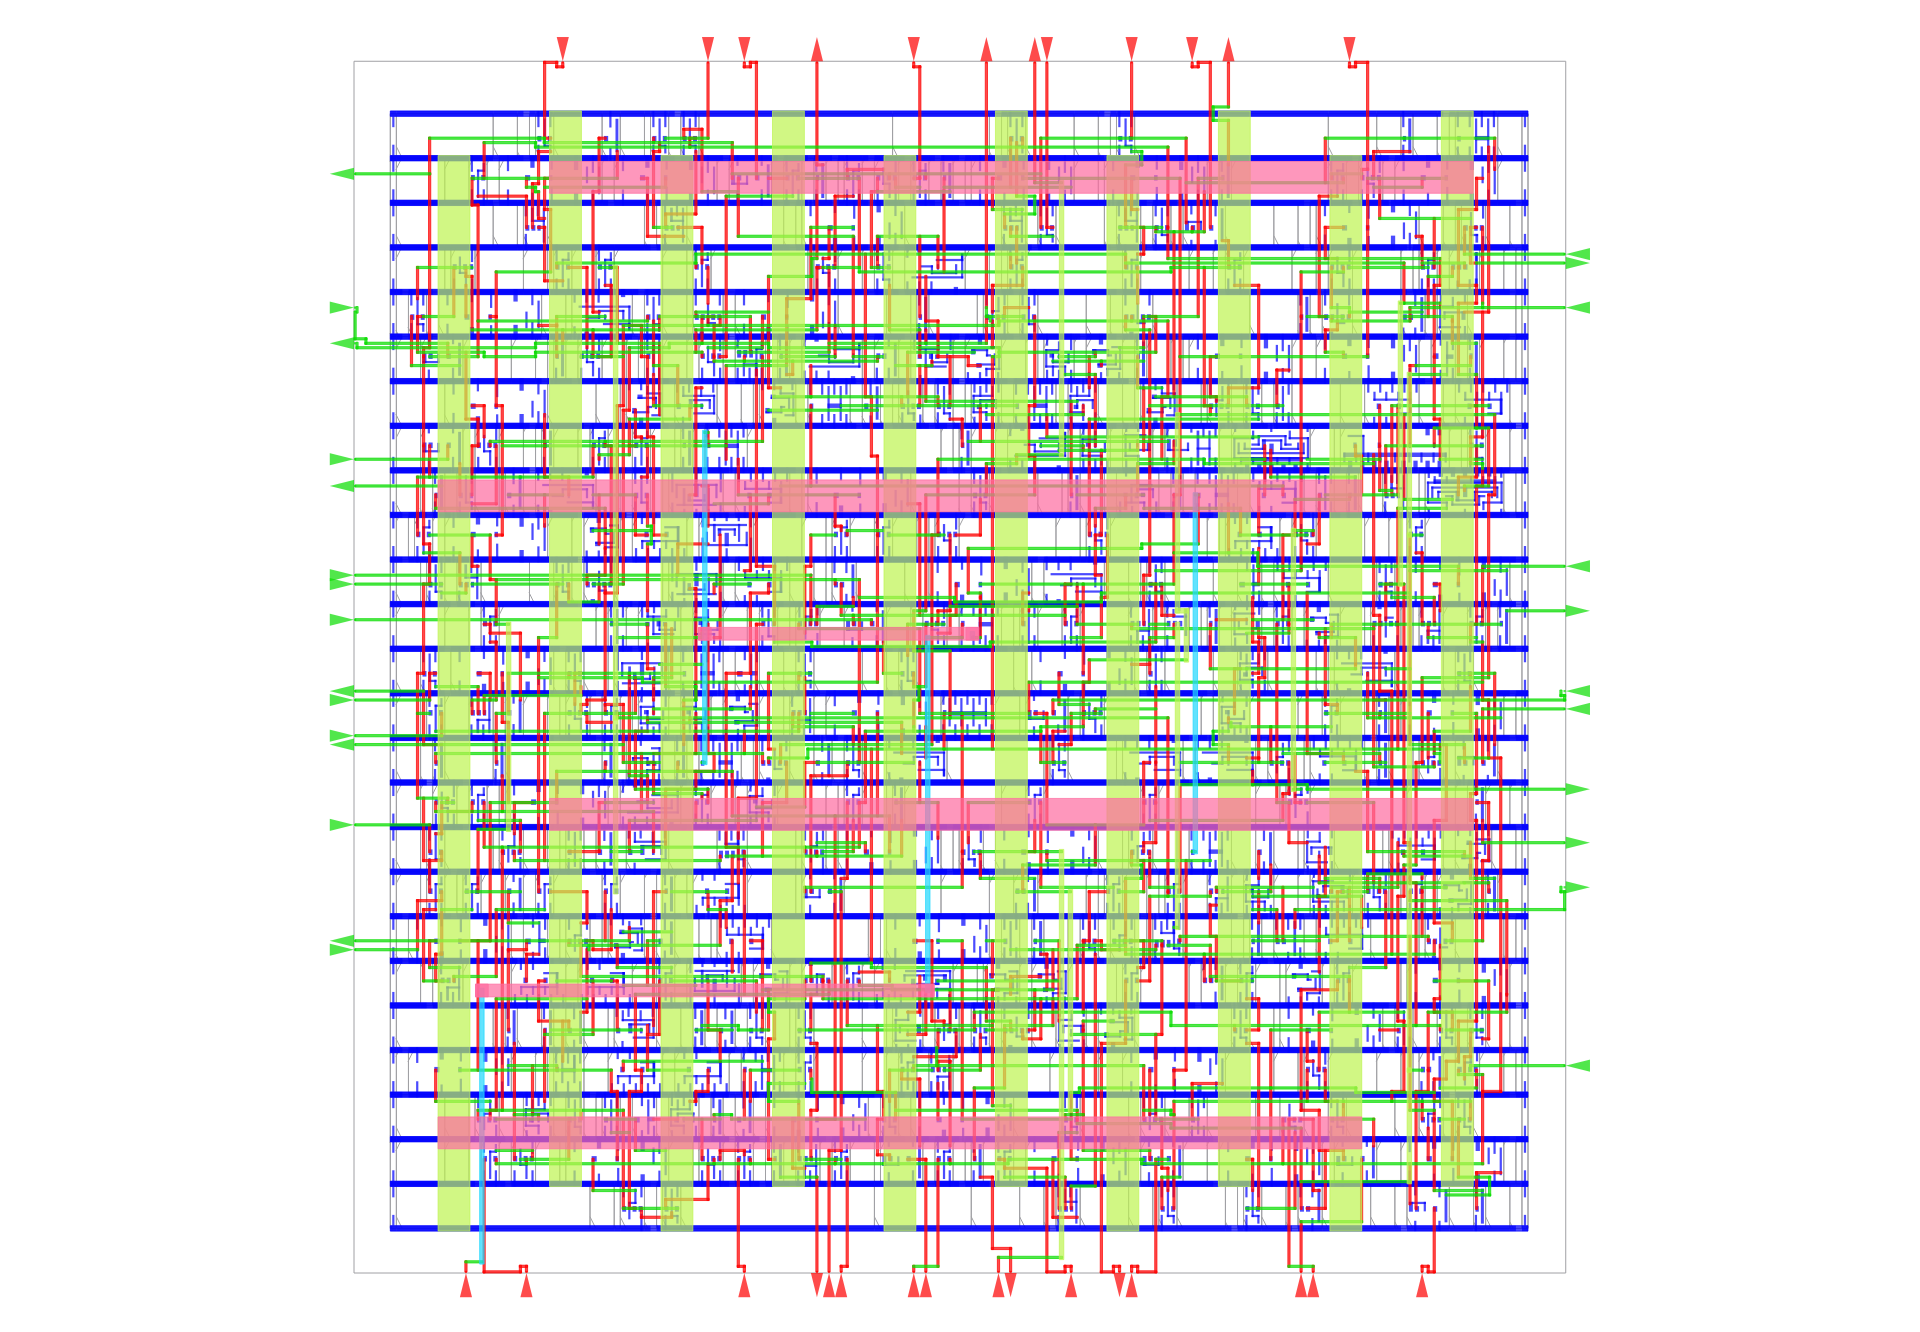
\includegraphics[height=112mm,trim=250 30 250 30,clip]{images/design.png}};

  \node[anchor=north west,text=black,text width=182mm,font=\bfseries\fontsize{12}{14.5}\selectfont] at (14mm,-196mm) {Learn to use \textcolor{openroadgreen}{OpenROAD} tooling for chip design steps \mbox{including:}};
  \checkitem{213mm}{Netlists, technology files, timing constraints}
  \checkitem{226mm}{Floorplanning, pin placement, and macros}
  \checkitem{239mm}{Global placement and legalization}
  \checkitem{252mm}{Clock-tree synthesis and timing repair}
  \checkitem{265mm}{Global routing, detail routing, and finishing}

  \node[anchor=north,inner sep=0] at (167mm,-210mm) {
\includegraphics[width=50mm]{qr.png}};
  \node[anchor=north,text=black,font=\bfseries\fontsize{8}{9.5}\selectfont] at (167mm,-262mm) {Read more on OpenROAD here!};

  \node[anchor=south,text=black,text width=182mm,align=center,font=\bfseries\fontsize{8.5}{10.5}\selectfont] at (105mm,-286mm) {Organized for and by PhD students at the \href{https://www.dm.uni-bonn.de/}{Research Institute for Discrete Mathematics}\\and \href{https://www.ftd.uni-bonn.de/}{Research and Technology Center for Detector Physics (FTD)}};

\end{scope}
\end{tikzpicture}
\null
\end{document}
